\chapter{Case Study}
\label{chapter: Case Study}

The substantiation to focus on Rozenburg and Heijplaat as case study areas, stems from the data availability and collection methods that are employed in these areas. With a dense network of data loggers and a comprehensive historical database, the study areas enable a thorough examination of the distribution of monitoring wells and the variation in groundwater levels across.

\section{Rozenburg}
The headland Rozenburg is notable for its eponymous village. Part of the headland has undergone extensive excavation measures and now serves the purpose of an industrial landscape. Prior to 2010, the village maintained its autonomy as Gemeente Rozenburg, but eventually merged into the larger City of Rotterdam. Positioned on the headland, the village finds itself in the inner dike area, enclosed by the industrial zones of \textit{Botlek} and \textit{Europoort}. The worlds of port and industrial activities as well as nature coexist. Therefore, part of the headland is called the \textit{“Groene Gordel” } \cite{port-of-rotterdam-no-date}. In the 1950s, the headland primarily functioned as an agricultural area with a dune and nature reserve \textit{“de Grote Beer” }on the western side. However, in the 1960s, major excavation measures took place to accommodate the development of \textit{Maasvlakte} and \textit{Europoort} industrial areas \cite{damme-jongsten-2008}. Given its location, Rozenburg faces a notable risk for flood events. The headland has an average ground level of +5.7 meters NAP \cite{visch-2022}, while the neighborhood itself has a much lower ground level, see figure \labelcref{AHNroz}. The strategic elevation differences reduces the village's vulnerability to potential flooding, particularly from the canal \textit{"Nieuwe Waterweg"} on the northern side of the district. Figure \labelcref{AHNroz} shows an elevation model of Rozenburg, based on a digital terrain model with a resolution of 0.5 meters. As can be seen from the figure, the neighborhood Rozenburg is located in the orange marked area with a dike ring in the red marked areas. \\
\begin{figure}[htbp]
    \centering
    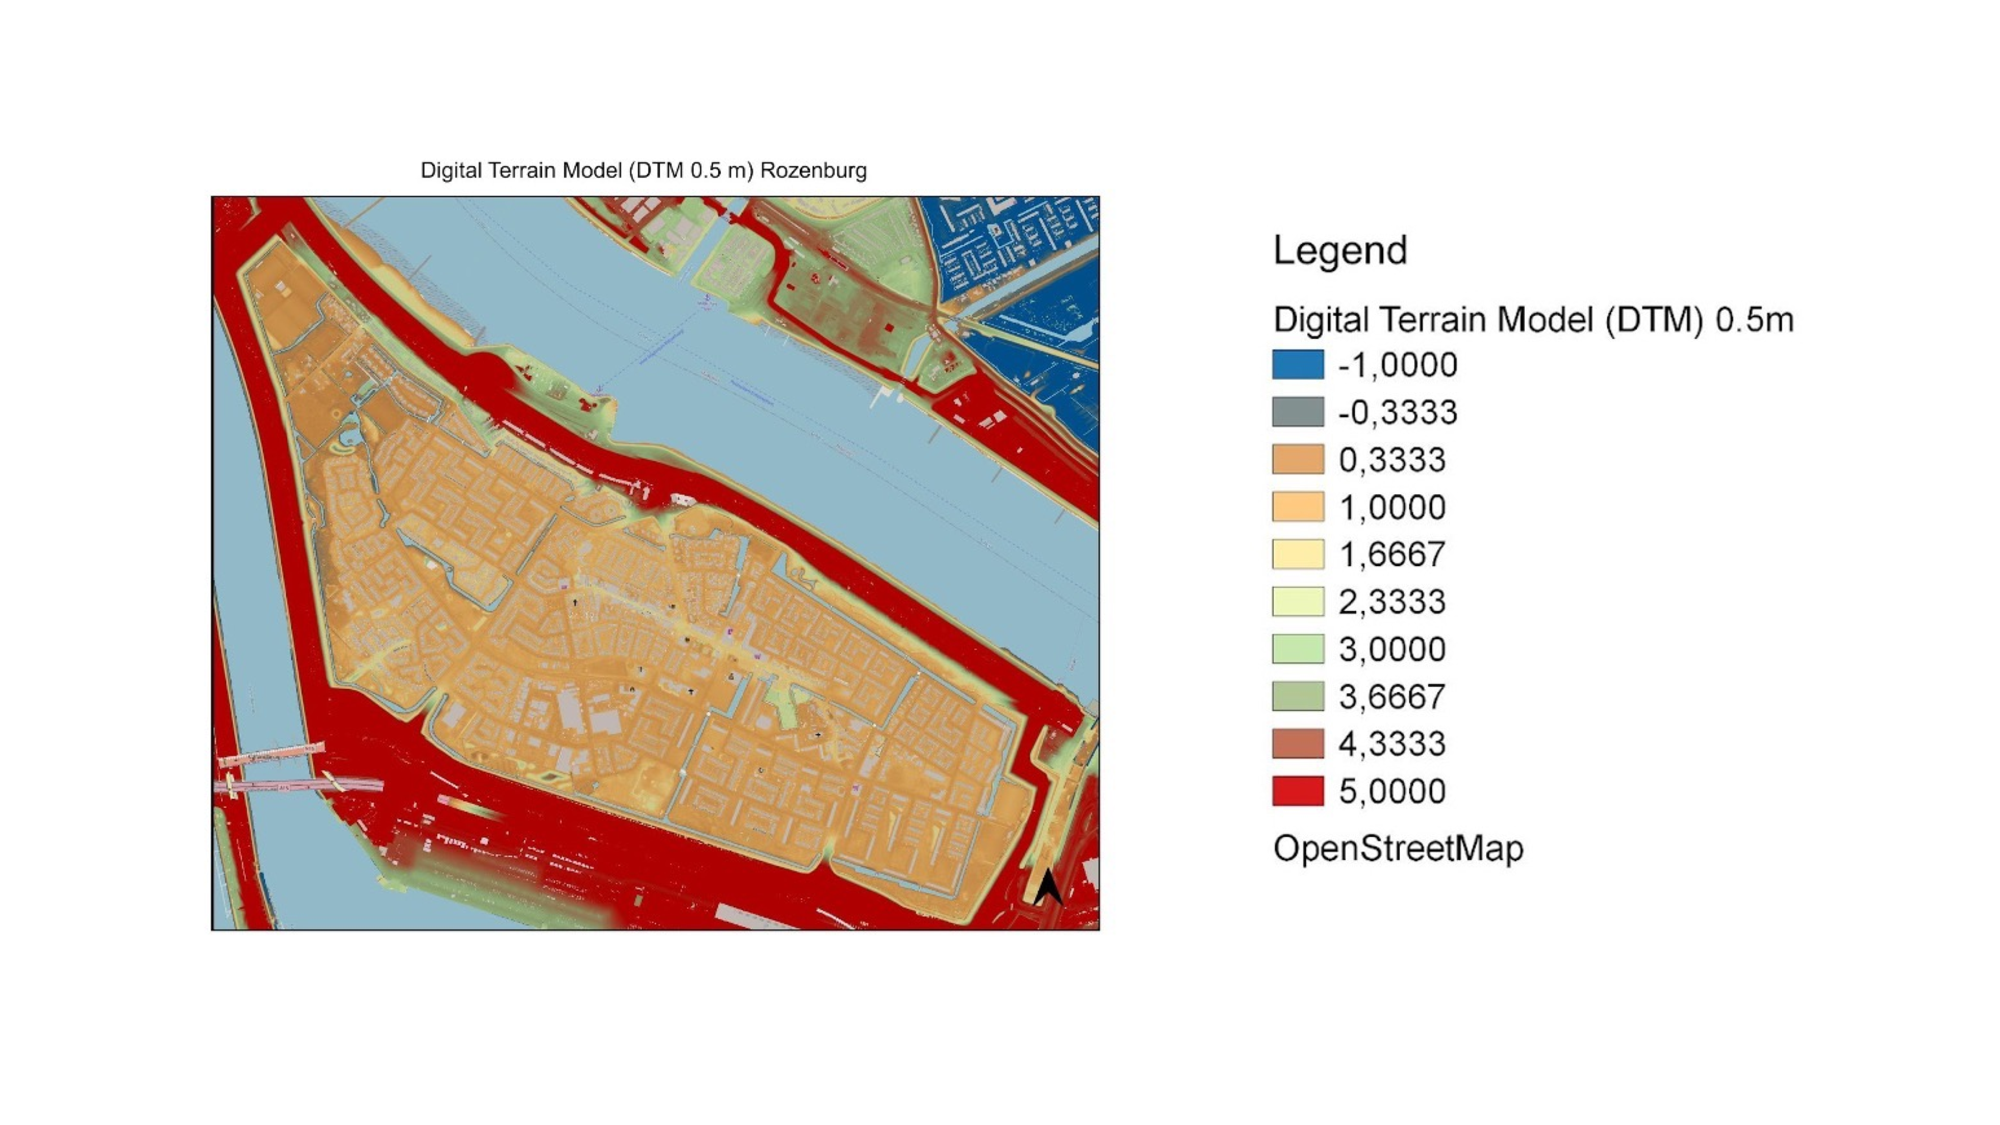
\includegraphics[width=0.80\linewidth]{figures/roz/ahnrozfig.pdf}
    \caption{Digital terrain model (DTM 0.5 m) for Rozenburg. Areas marked in red indicate locations with the highest elevation, while orange marked areas indicate locations with the lowest elevation.}
    \label{AHNroz}
\end{figure}\\
Regarding the geology of the area, the first 22.91 meters are a Holocene formation that consists of sandy clay, medium-fine sand, clay, peat, and coarse sand, see figure \labelcref{georoz}. The presence of these sediments suggest a varied deposition environment; fluvial and marine processes. The diverse grain sizes of the sediment and the presence of an organic peat layer could indicate that infiltration rates can be varying and thus affect groundwater recharge and storage. Underneath the Holocene layer, a layer of about 1.46 meters of the formation of Kreftenheye is present, see figure \labelcref{georoz}. The formation consists of medium-coarse sand, little sandy clay, fine sand and cobbles with traces of clay and peat. The composition of the second formation indicates a more permeable layer, in comparison with the top Holocene formation. This can also be explained by larger grain sizes, which allows for groundwater movement and possible occurrence of an aquifer \cite{janssen-2005}. 
\newpage
\noindent
Collectively, the upper Holocene formation introduces a varied texture, ensuring heterogeneous permeability that affects groundwater flow and storage. The heterogeneity arose from the varied sediment composition, impacting the infiltration rate and groundwater dynamics. On the other hand, the Kreftenheye formation characterizes itself as a permeable formation, which is the result of the medium-coarse sand and cobbles. Given the focus of the research study on phreatic monitoring wells, only the Anthropocene and Holocene formation are considered. However, for this specific drilling location, no information regarding the Anthropocene formation is available through BRO GeoTOP v1.6. This can also be seen in figure \labelcref{georoz}, the drill site profile called \textit{"Lithoklasse"} in the middle of the figure explains a combination of clayey-sand, sandy-clay and loam in the first 20 meters of the profile. 

\begin{figure}[htbp]
    \centering
    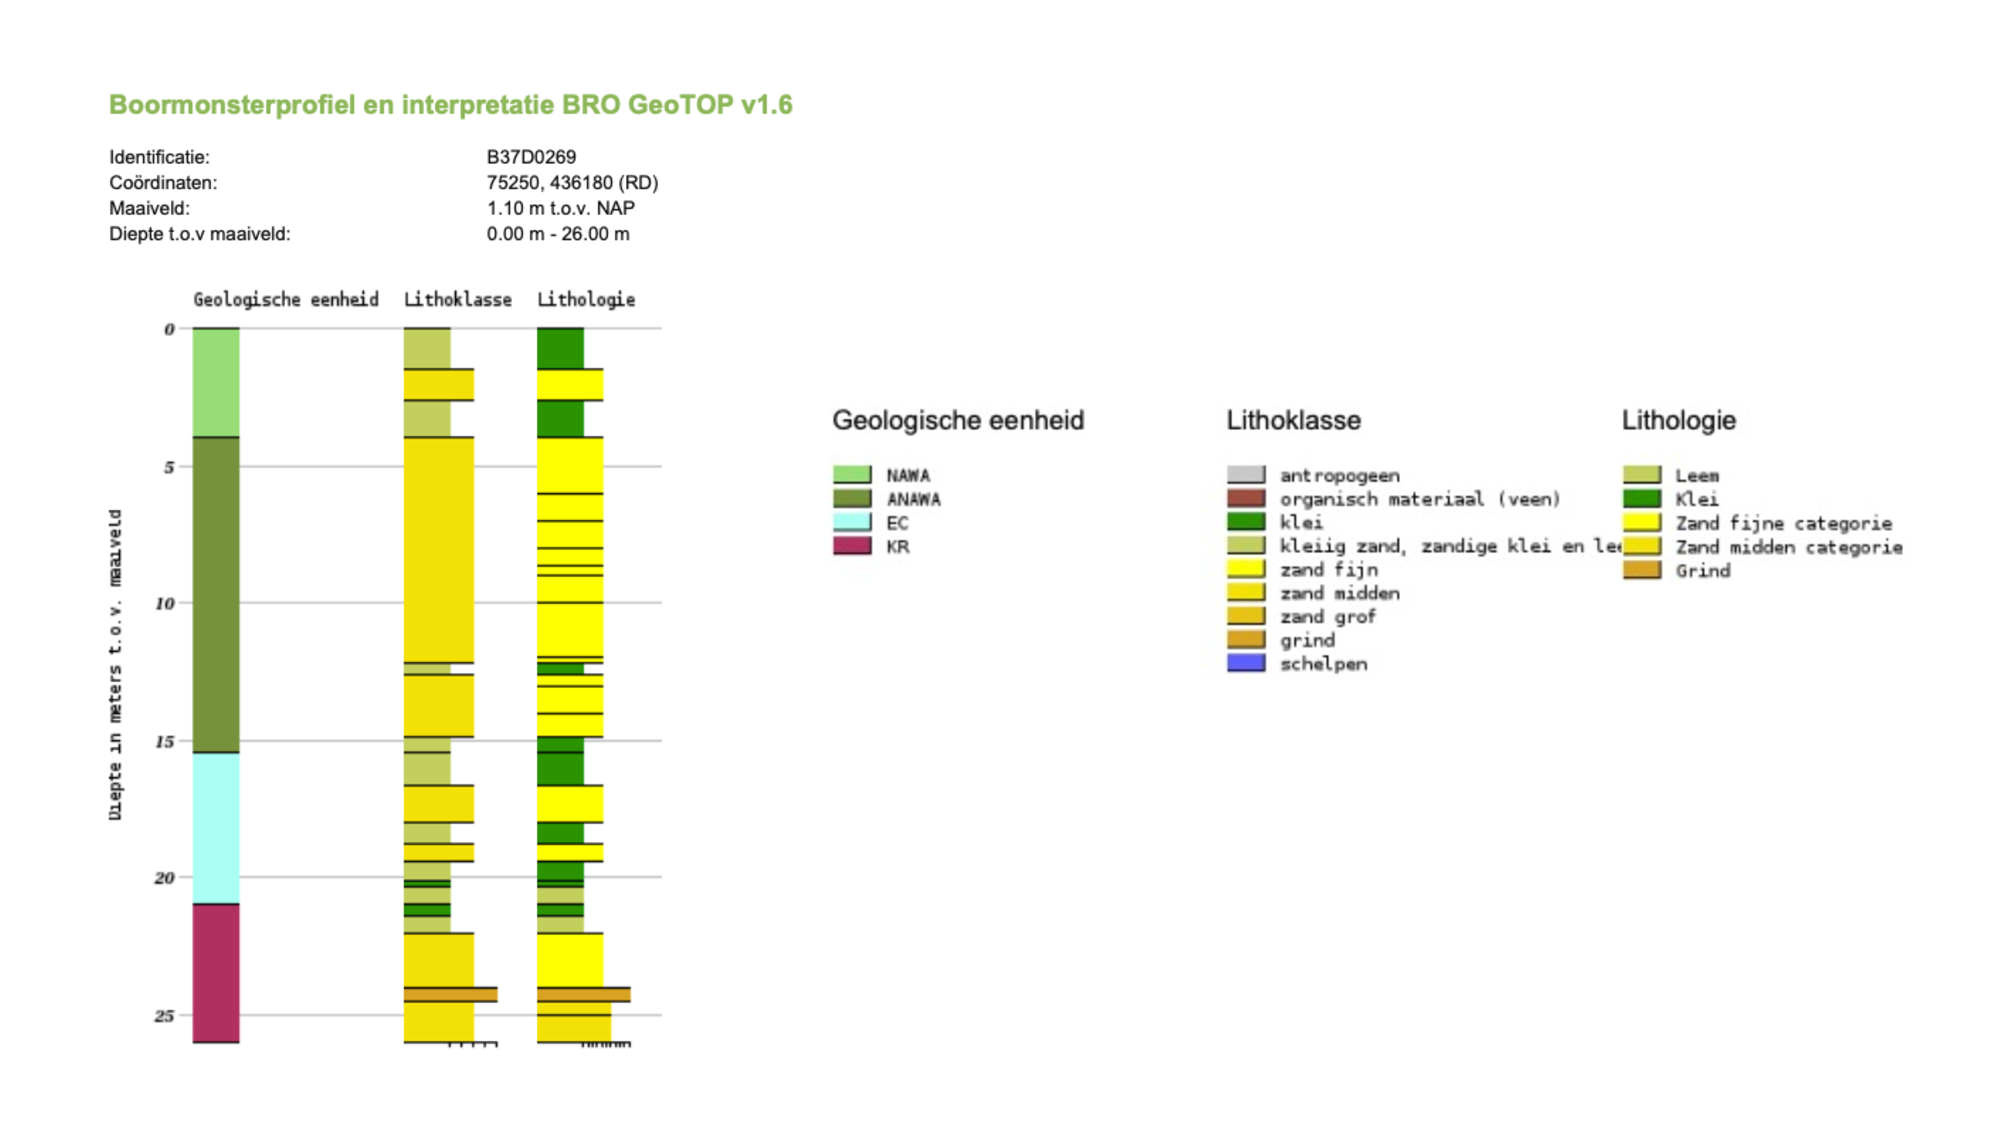
\includegraphics[width=0.75\linewidth]{figures/roz/rozboor.pdf}
    \caption{Profile of drill site profile with geological formations for the location x: 75250; y: 436180 \cite{tno-geologische-dienst-nederland-2023}.}
    \label{georoz}
\end{figure}\\
\noindent
The location of the exact drill profile is shown in figure \labelcref{drillroz}. As can be seen in the figure, the location is in the southwestern side of the neighborhood, close to the connecting road. Only one drilling profile is considered, since this is the only drill profile that is present within the boundaries of the neighborhood.

\begin{figure}[htbp]
    \centering
    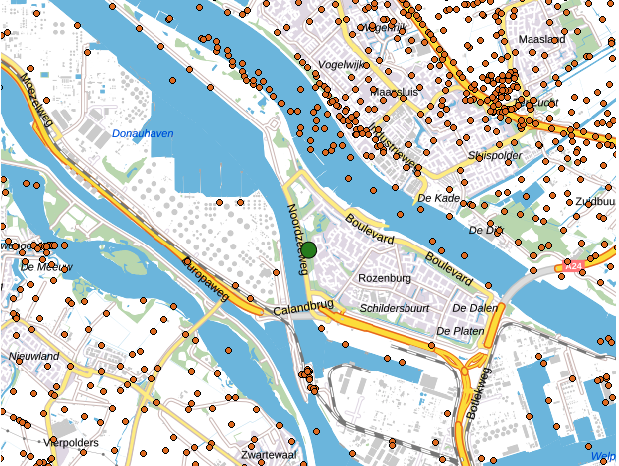
\includegraphics[width=0.60\linewidth]{figures/roz/boor.png}
    \caption{Precise location for the drilling profile by the coordinates x: 75250, y: 436180 \cite{tno-geologische-dienst-nederland-2023}.}
    \label{drillroz}
\end{figure}
\newpage
\noindent
As stated by CBS, the total surface area of Rozenburg counts up to 411 hectares in total, of which 324 hectares is made of land. Rozenburg has 29 active, phreatic monitoring wells, meaning one monitoring well/11.17 hectares. In figure \labelcref{beforeroz}, a geographical representation of the neighborhood Rozenburg is displayed. Points of interest are the blue marked points, which indicate the available phreatic monitoring wells in the neighborhood.
\begin{figure}[htbp]
    \centering
    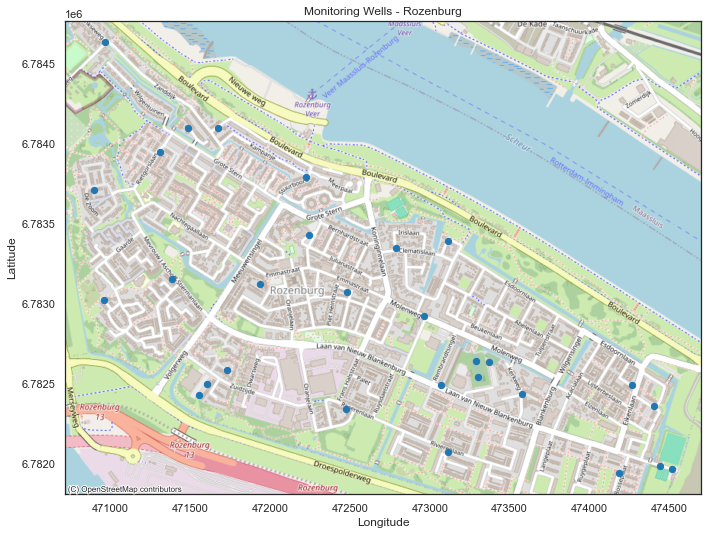
\includegraphics[width=0.70\linewidth]{frontmatter/Rozenburg-fig/Before.png}
    \caption{Groundwater monitoring network in Rozenburg. Based on EPSG:28992/Amersfoort RD New.}\label{beforeroz}
\end{figure}
\newpage
\section{Heijplaat}
Since the mid-15th century, the hamlet \textit{"de Heij" }has been located at the northern side of the neighborhood Charlois. At the north of the hamlet, the creek \textit{"de Koedood" }flew into the Meuse. However, years later, an industrial area called\textit{"de Heijsehaven"} was constructed at that site, where an artificial sand formation was formed as well. Only at the beginning of the 20th century, the idea of the garden village arose  \cite{sebregts-2019}. Throughout the years, the village became more isolated because of the extension of the industrial areas \cite{port-of-rotterdam-2008}. Figure \labelcref{ahnheij} shows that Heijplaat is still surrounded by industrial areas and water outside the dike ring. Access to Heijplaat is solely possible through one entrance road, the \textit{"Waalhavenweg"} \cite{milieudienst-rijnmond-2023}. Figure \labelcref{ahnheij} describes a digital terrain model with a resolution of 0.5 meters for the neighborhood. From the figure it can be seen that the neighborhood is located on a constant level of about 2-3 meters NAP. 
\begin{figure}[htbp]
    \centering
    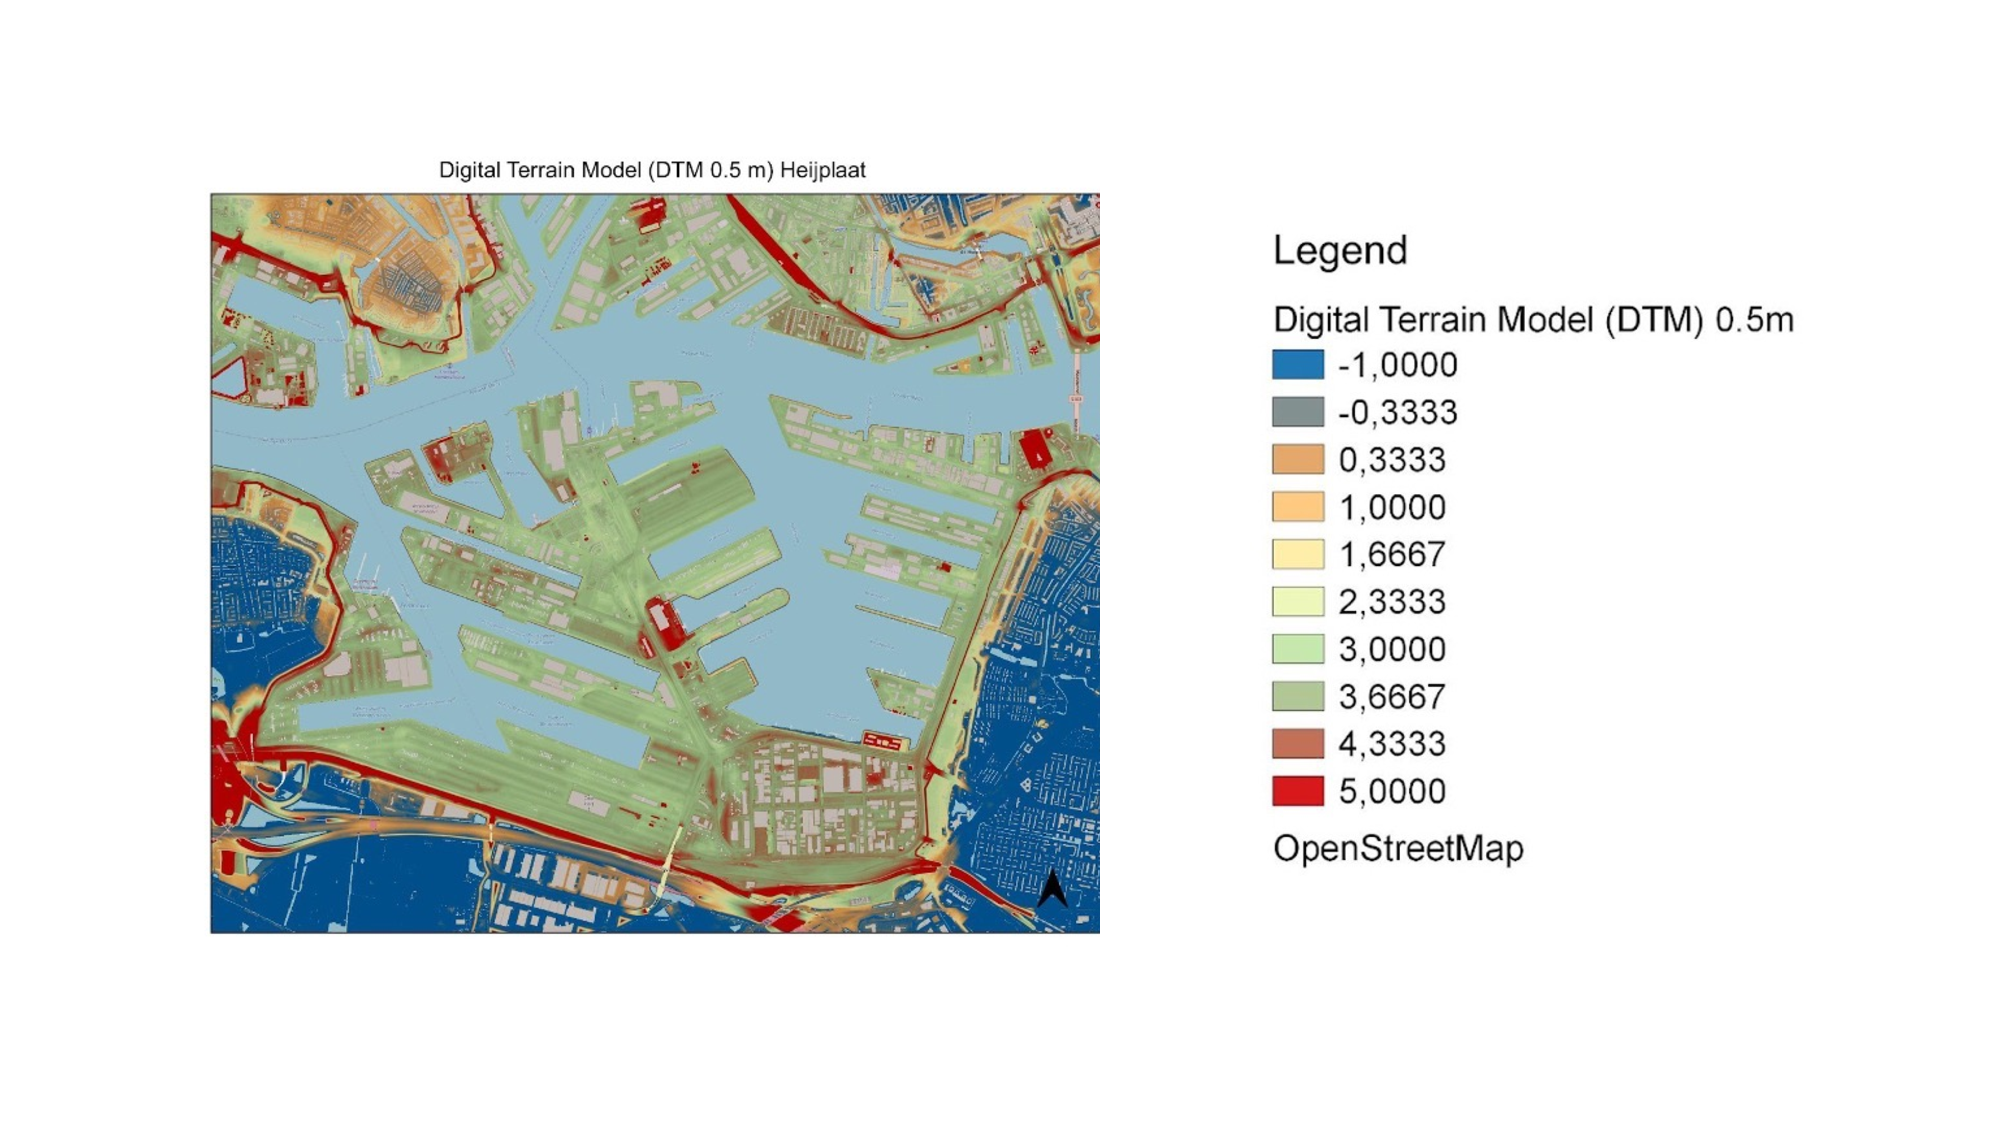
\includegraphics[width=0.80\linewidth]{figures/heij/ahnheijfig.pdf}
    \caption{Digital terrain model (DTM 0.5) for Heijplaat. Areas marked red indicate the locations with the highest elevation, while blue marked areas indicate locations with the lowest elevation.}
    \label{ahnheij}
\end{figure}\\
\\
%At the end of 2023, it emerged that the neighborhood experienced issues with the establishment of a new waste management firm. Additionally, water-related problems have been documented in the historic center as well. Construction initiatives have been proposed to address these issues with a focus on replacing the sewage system as a solution to the water-related inconveniences \cite{gemeente-rotterdam-2023}. \\
\\
Figure \labelcref{geoheij} shows the lithology of Heijplaat. The subsurface in the eastern part consists of deposits from the formations Dunkirk III, Dunkirk I, and peat. A stratified geology is suggested with peat deposits present in areas with a high organic content. The peat deposits could influence water retention and filtration properties. On the western part of Heijplaat, however, the subsurface is characterized by the Dunkirk III formation atop a peat layer. The under-layer of peat indicates wet conditions in the past, referring to the relocation of the Riederwaard dike, which could influence the groundwater dynamics with layers of varying hydraulic properties \cite{gemeente-rotterdam-2013}. In the period of the 10-12th century, the peat landscape has been drained which altered the landscape significantly. This showed itself through ground level reductions, necessitating dike construction. The manipulation of the landscape impacted and reshaped the groundwater recharge, flow and storage ability in the area. The upper Anthropocene layer is characterized  by sand, fine to coarse clay, silty to sandy humic, and a layer of debris of about 2.3 meters thick in total, see the gray unit in the first site profile of figure \labelcref{geoheij} \cite{tno-geologische-dienst-nederland-2023}. Overall, the area is marked by historical land alterations and complex, stratified geology, which influences the groundwater recharge rate, flow, and storage capacity in the neighborhood of Heijplaat. This specific drilling location is chosen, because it lies in the south of the area and is not located on the eastern side of the railway that crosses the neighborhood. The drill site profile called \textit{"Lithoklasse"} in the middle of the figure explains a combination of fine-sand, clayey-sand, sandy-clay, and loam. 
\newpage
\begin{figure}[htbp]
    \centering
    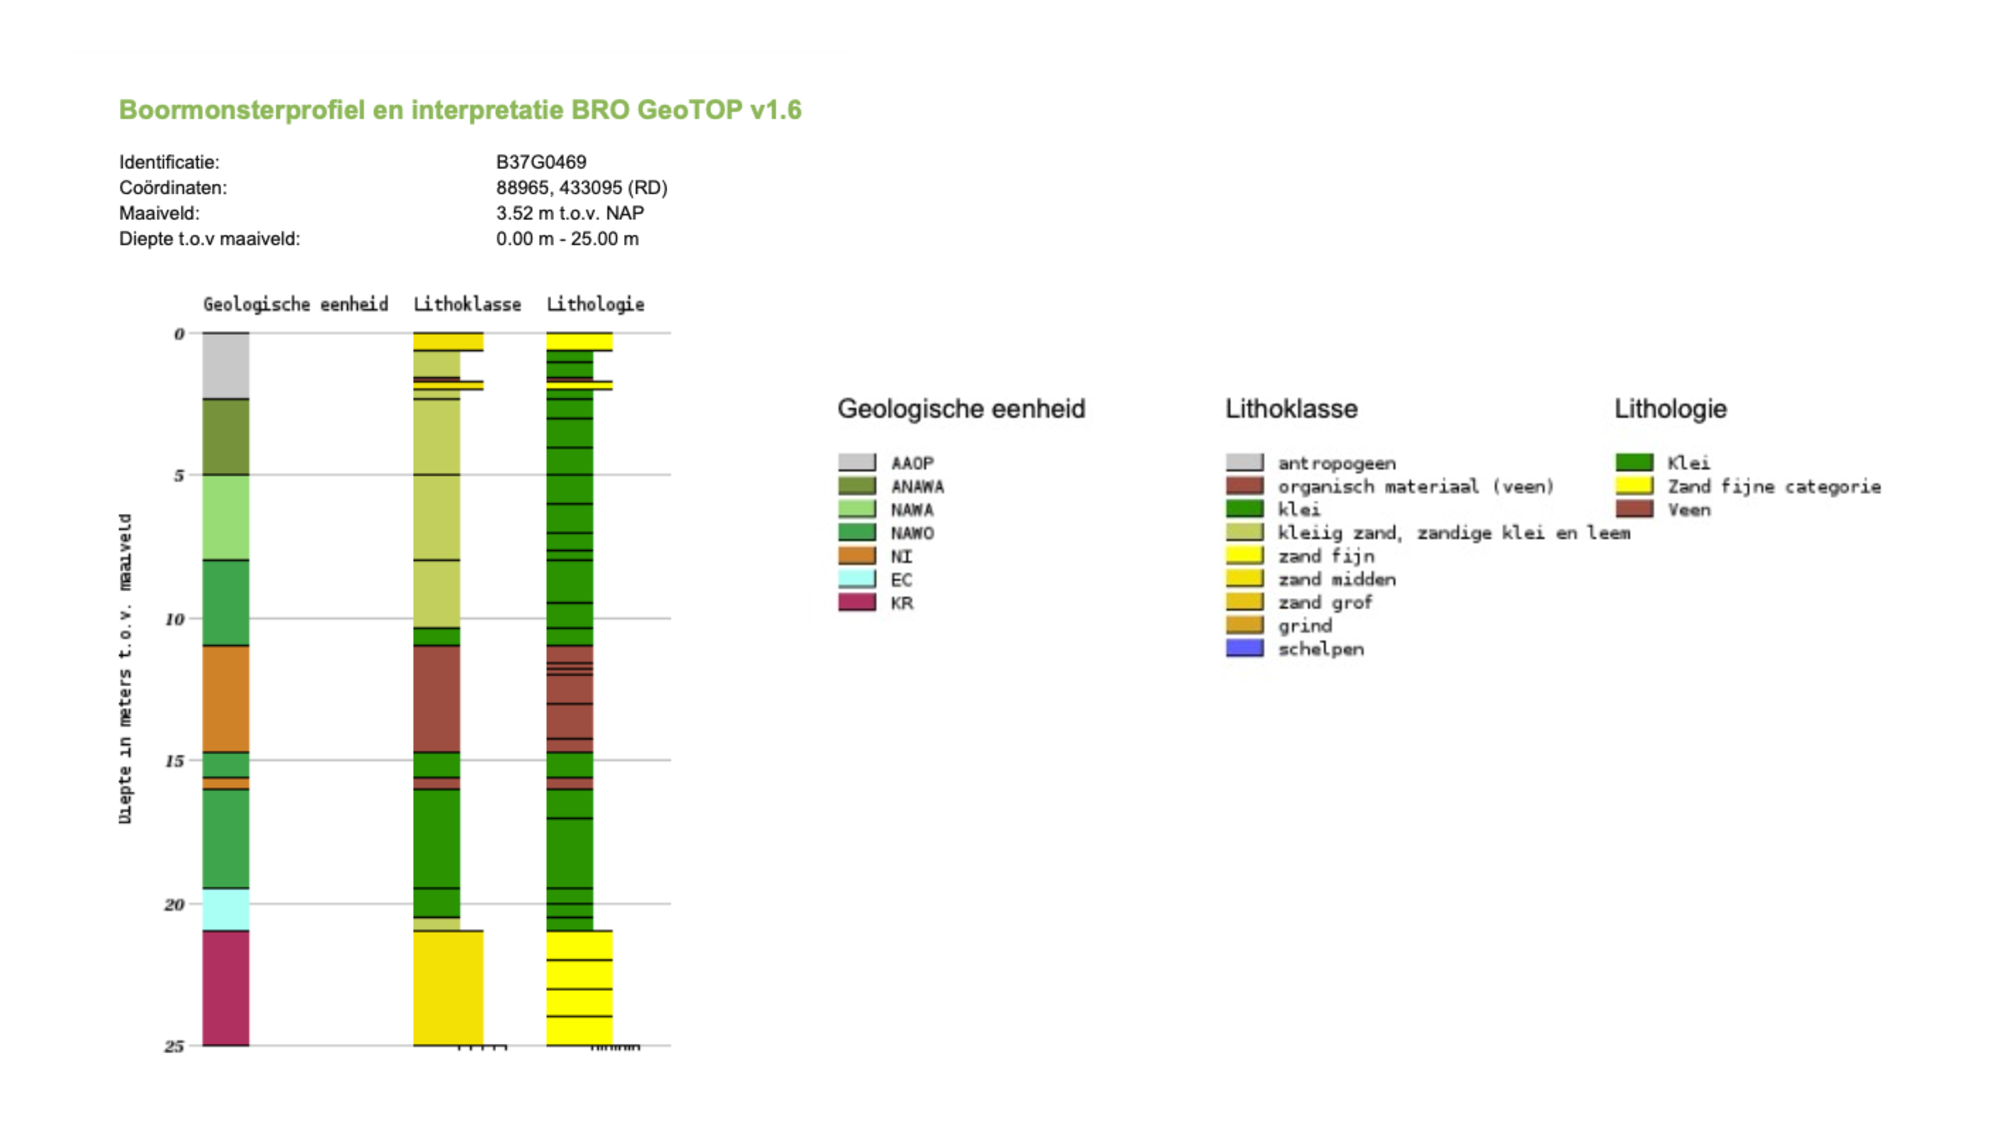
\includegraphics[width=0.75\linewidth]{figures/heij/heijboor.pdf}
    \caption{Profile of drill site profile with geological formations for the location x: 88529; y: 433870 \cite{tno-geologische-dienst-nederland-2023}.}
    \label{geoheij}
\end{figure}
The location of the exact drill profile is shown in figure \labelcref{drillheij}. As can be seen in the figure, the location is on the southern side of the neighborhood.
\begin{figure}[htbp]
    \centering
    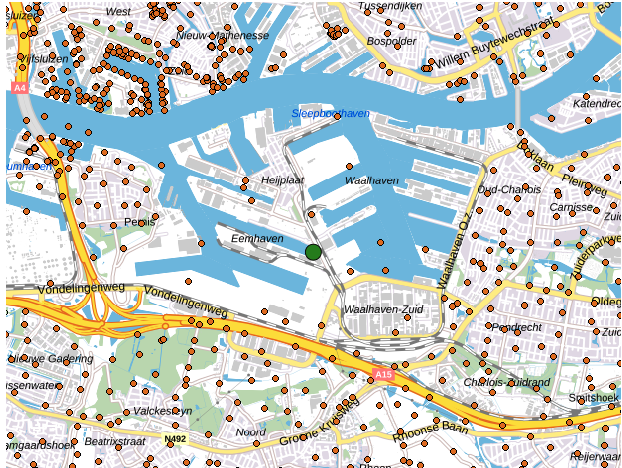
\includegraphics[width=0.60\linewidth]{figures/heij/boor.png}
    \caption{Precise location for the drilling profile by the coordinates x: 88529, y: 433870 \cite{tno-geologische-dienst-nederland-2023}.}
    \label{drillheij}
\end{figure}\\
\noindent
The total surface area of Heijplaat counts up to 39 hectares in total, of which 39 hectares are also made of land \cite{centraal-bureau-voor-de-statistiek-2020}. In Heijplaat, one monitoring well is present per one well/2.78 hectares according to \cite{centraal-bureau-voor-de-statistiek-2020}. Figure \labelcref{beforeheij} visualizes a geographical representation of the neighborhood Heijplaat, part of Charlois. Points of interest are the blue marked points. They indicate the available phreatic monitoring wells in Heijplaat. 

\begin{figure}[htbp]
    \centering
    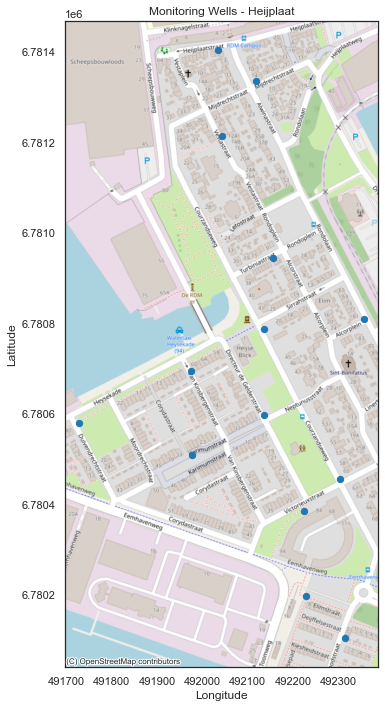
\includegraphics[width=0.60\linewidth]{frontmatter/Heijplaat-fig/Before.png}
    \caption{Groundwater monitoring network in Heijplaat. Based on EPSG:28992/Amersfoort RD New.}
    \label{beforeheij}
\end{figure}
